\subsection{Communication Patterns}
In this paper we demostrate data movement performance of our OPTIQ framework and existing MPI's routines on the following communication patters:

\begin{figure}[ht]
\vspace{-0.1in}
\centering
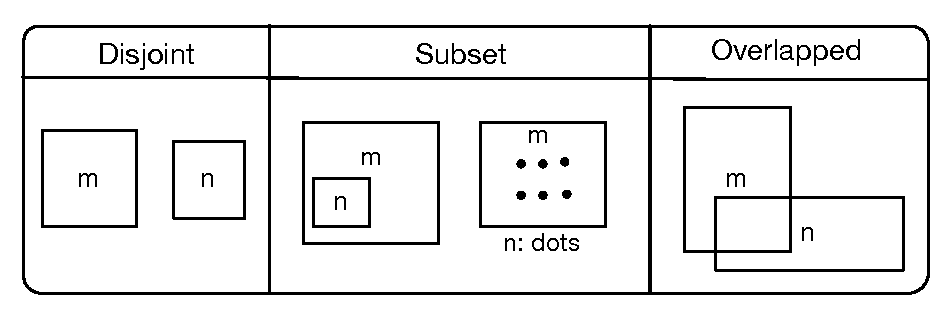
\includegraphics[scale=0.55]{figures/patterns.pdf}
\vspace{-0.1in}
\caption{Communication patterns}
\vspace{-0.1in}
\label{fig:patterns}
\end{figure}

\begin{itemize}
\item Disjoint sets: is many-to-many communication pattern where the sources and destinations are separated. It is a typical pattern in many applications.
\item Overlap: is a many-to-many pattern that sources and destinations are overlapped sets. CESM uses this communication patterns for its coupling communications.
\item Subset: is a many-to-many pattern that sources or destinations are subset of the other. The patterns can be found CESM or in I/O aggregation.
\end{itemize}

We carried a set of experiments to study the system's behavior in various patterns and demontrate throughput improvement.
